\documentclass[11pt]{article}

\usepackage[utf8]{inputenc}
\usepackage[T1]{fontenc}
\usepackage{graphicx}
\usepackage[linktocpage=true]{hyperref}

\usepackage{mathpazo}

\begin{document}
\begin{titlepage}
	\newcommand{\HRule}{\rule{\linewidth}{0.5mm}}
    \begin{center}

    	\textsc{\LARGE Alabama Liquid Snake}\\[0.8cm]
    	\textsc{\Large University of Pretoria}\\[0.5cm]
    	\textsc{\large Epi-Use}\\[0.5cm]

    	\HRule\\[0.4cm]

    	{\huge\bfseries Botic - Privacy aware chatbot}\\[0.2cm]

    	{\huge User Manual}\\[0.2cm]

    	\HRule\\[0.5cm]

	    \textsc{Justin Grenfell} - u16028440 \\[0cm]
	    \textsc{Peter Msimanga} - u13042352 \\[0cm]
	    \textsc{Alicia Mulder} - u14283124 \\[0cm]
	    \textsc{Kyle Gaunt} - u15330967 \\[0cm]
	    \textsc{Lesego Mabe} - u15055214 \\[0cm]

    \end{center}
\end{titlepage}
\tableofcontents
\newpage
\section{Introduction/System Overview}
\begin{flushleft}
	Botic is a customer service communication chat service that uses artificial intelligence to handle user requests regarding account information or company protocols, without compromising the user’s privacy or personal information.\\[0.5cm]
	Information provided by the user is reviewed and analyzed before transmission to ensure that no unnecessary private information is sent over the Internet. This will help reduce risk for users that may not be aware of privacy protection techniques or methods and will ensure that the company is not liable for any illegal gathering of information according to local and international laws.\\[0.5cm]
	There are three primary users that the system caters for, namely: the client, the client representative and the administrator.
	The client is catered for by providing a secure and intelligent chat system that can answer their queries quickly and effectively all the while protecting their privacy as far as possible.\\[0.5cm]
	The client representative makes use of a platform that allows them to respond to requests that the artificial intelligence system is not sure how to handle, whilst also ensuring that no private information is compromised.\\[0.5cm]
	Lastly, an administrator is given a management suite that allows for custom configuration of the system to ensure that each company is provided a flexible and effective software solution.\\[0.5cm]
\end{flushleft}
\subsection{System Configuration}
\begin{flushleft}
	The equipment, communications and networks used by the system are designed to be as interchangeable as possible to allow for each individual company to incorporate their own systems and technologies for maximum cohesion.\\[0.5cm]
	It is important to note that no core components will be interchangeable, only those components that do not affect the core functionalities of the system (i.e. email services and login management).\\[0.5cm]
	\textbf{In the case of the client:} the device will connect to the online Heroku component. That component will send the client's query through to the server which houses the company specific trained neural network. An appropriate response will be formulated. Depending on the response, it will either be forwarded to a client representative or sent back to the client.\\[0.5cm]
	\textbf{In the case of the client representative:} the device will connect to the online Heroku component which will forward a response that the company specific trained neural network was unable to respond to. The client representative will then review the case and provide the system with the correct response to send through to the client.\\[0.5cm]
\end{flushleft}
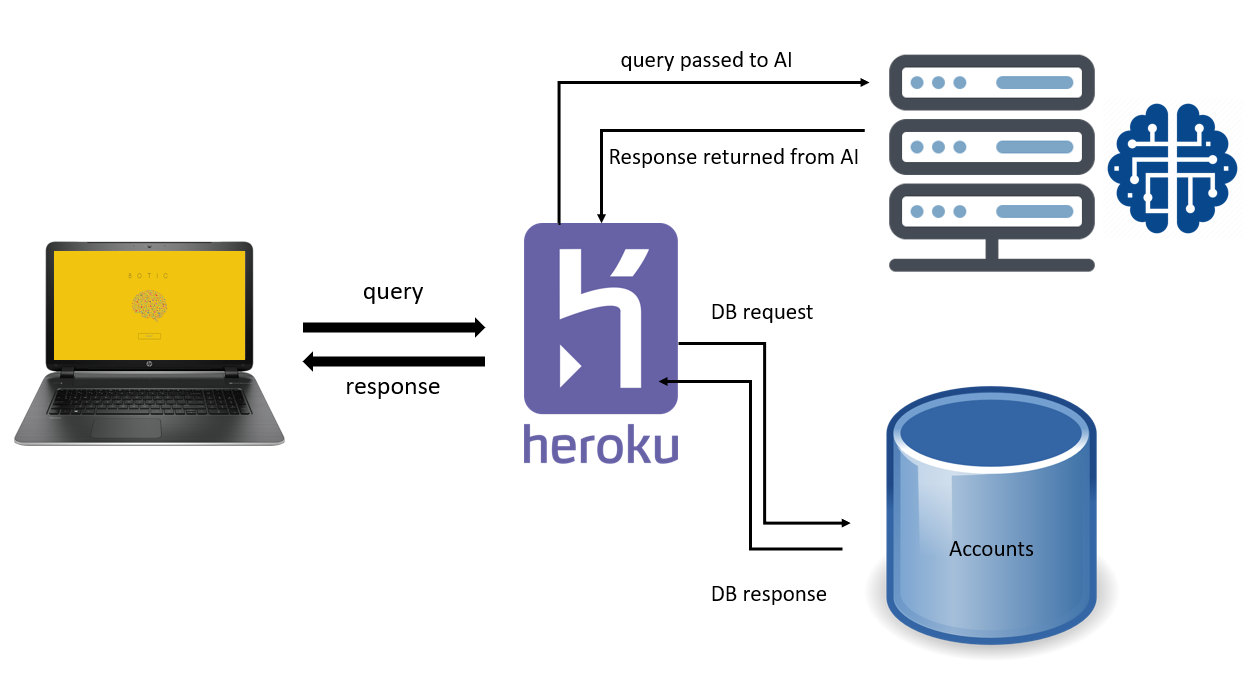
\includegraphics[width=1.0\textwidth]{Diagram1.PNG}

\subsection{Installation}
\begin{flushleft}
	The system will be packaged as a binary file which will then be extracted onto the client's server as part of deployment. In this way, the client can build their own system environment using their preferred technologies.\\[0.5cm]
	Users will be required to provide a valid license token which will then validate and activate the files. If an invalid or expired token is detected, the client will be denied access to the system until their license is renewed.\\[0.5cm]
\end{flushleft}
\section {Getting Started}
\begin{flushleft}
	Once installed, follow the confirmation email sent to the email used to register with Botic. The email will contain a unique key which should be entered into the “Registration Token” field. Once done, the system will confirm the token and the user will be taken through the setup process.
\end{flushleft}
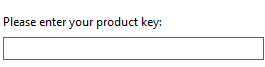
\includegraphics[width=1.0\textwidth]{ProductKey.png}

\begin{flushleft}
	As default, the account associated with the email used to register will be set as the system administrator. To add a new user, click “Add user”.
\end{flushleft}
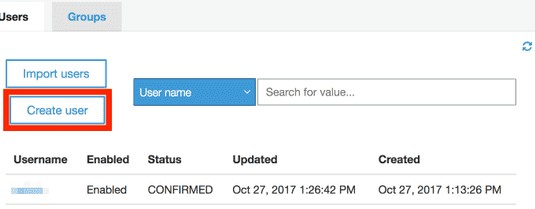
\includegraphics[width=1.0\textwidth]{CreateUser.jpg}

\begin{flushleft}
	Fill in the necessary fields. Once complete, click “Add user”. The new user has now been added.
\end{flushleft}
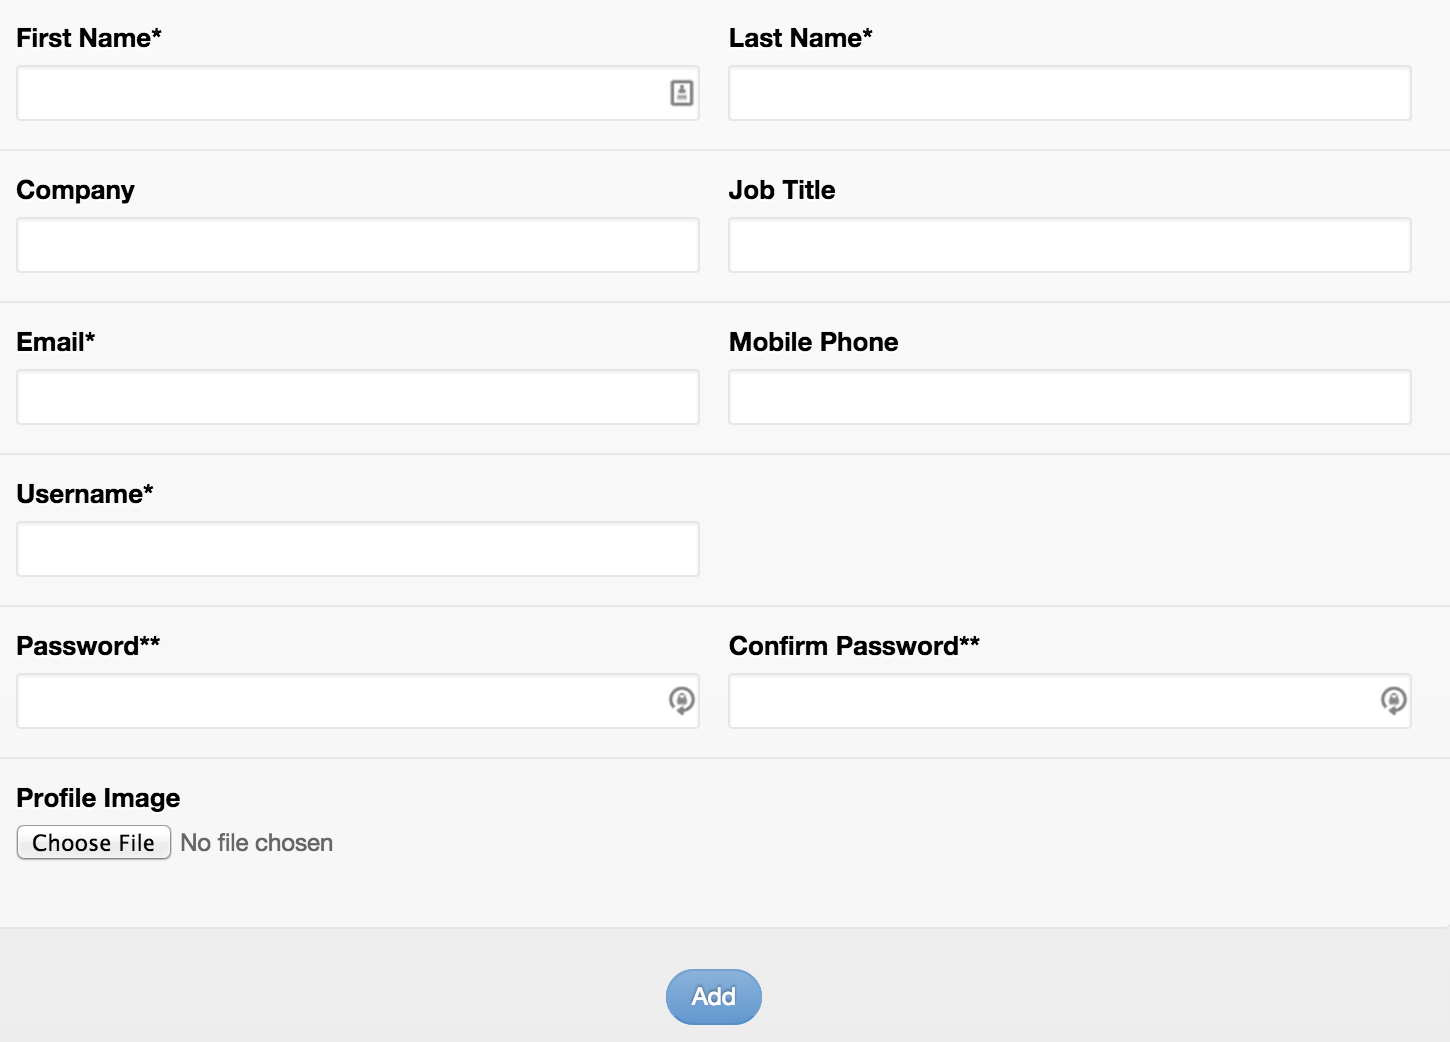
\includegraphics[width=1.0\textwidth]{AddUserForm.png}

\begin{flushleft}
	To request a new password, click “Sign in” followed by “Forgot password”. Follow the steps and an email will be sent to the associated account with a link to change the password.
\end{flushleft}
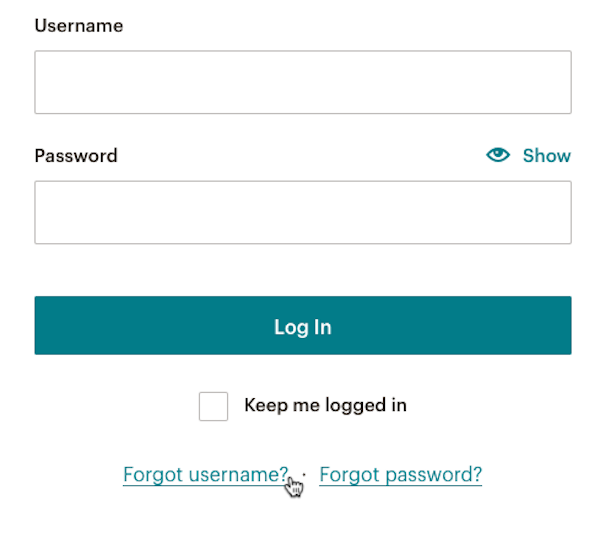
\includegraphics[width=1.0\textwidth]{Login.png}

\begin{flushleft}
	Once initiated, the system will require basic setup which can be done through the “Admin Page”.
\end{flushleft}

\section{Using the System}
\begin{flushleft}
	To access the chat service, navigate to http://botic-frontend.herokuapp.com/ and click “Chat”.
\end{flushleft}
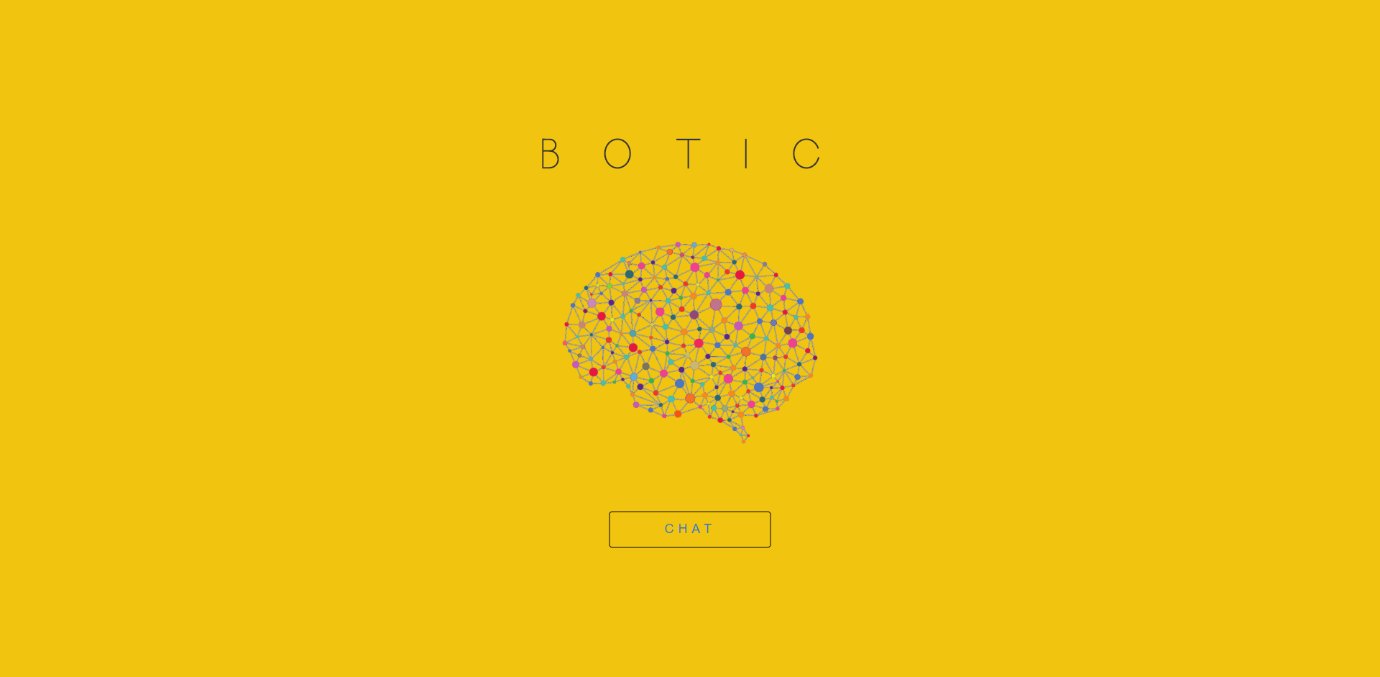
\includegraphics[width=1.0\textwidth]{Landing.png}

\begin{flushleft}
	Read through the User Agreement. Once complete, click on “Accept”.
\end{flushleft}
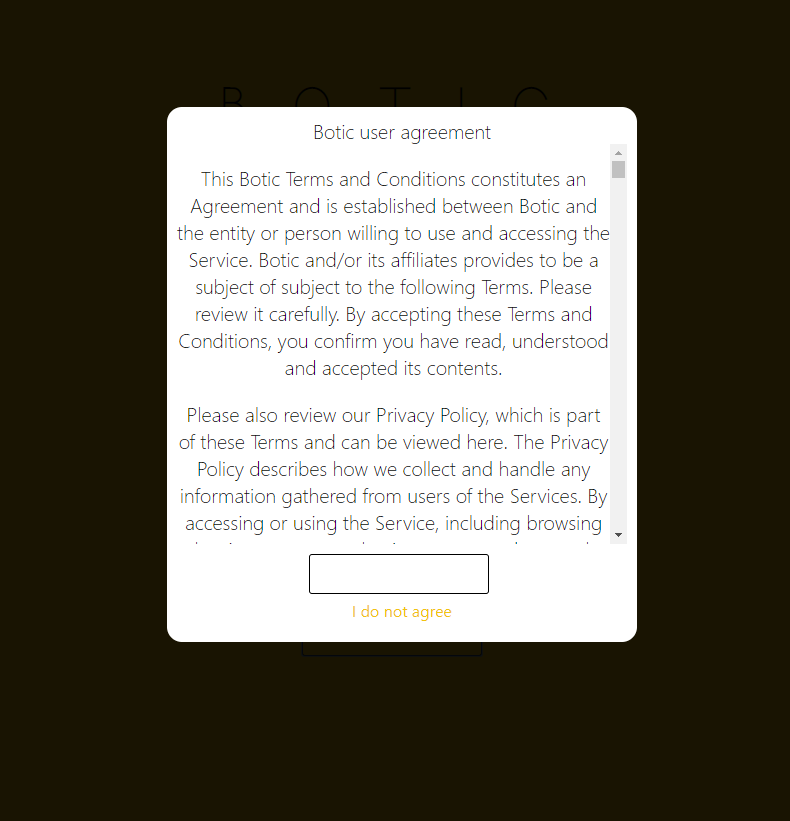
\includegraphics[height=0.91\textwidth]{UserAgreement.png}

\begin{flushleft}
	You will be redirected to the chat page.
\end{flushleft}
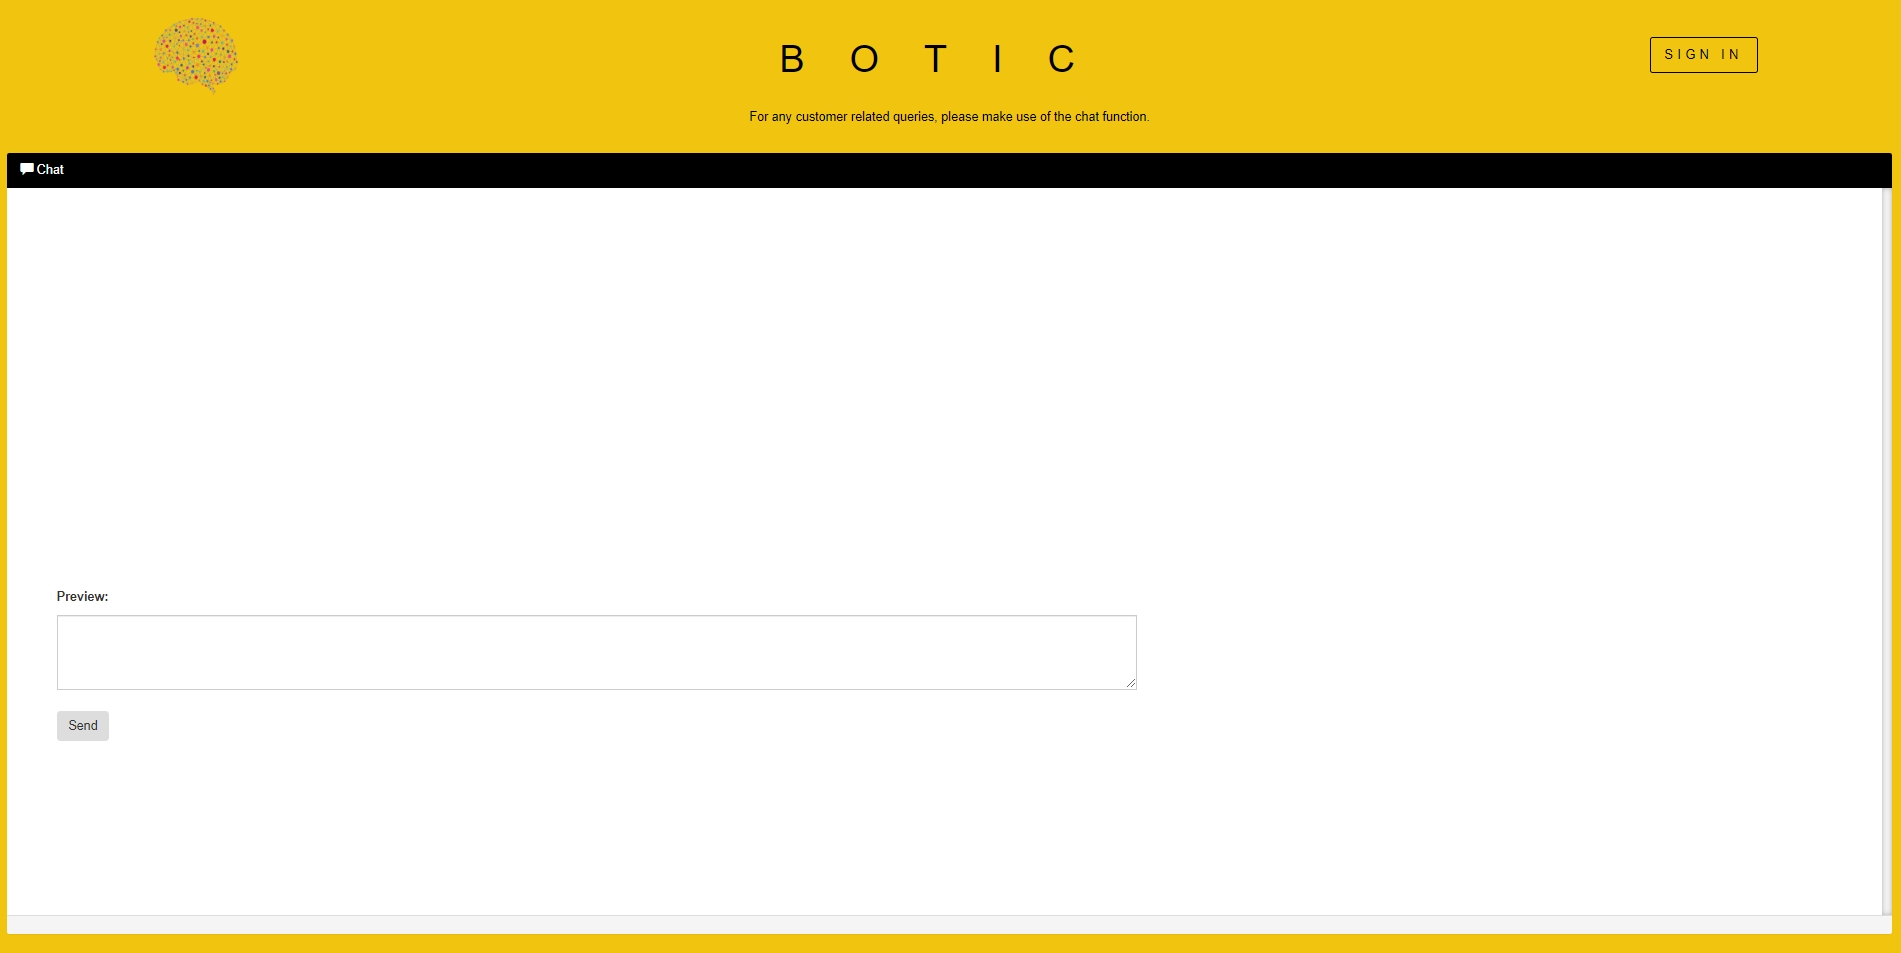
\includegraphics[width=1.0\textwidth]{ChatPage.png}

\begin{flushleft}
	Type your query into the text field, your text will be reviewed and any information that may prove to be a risk will be highlighted.
\end{flushleft}
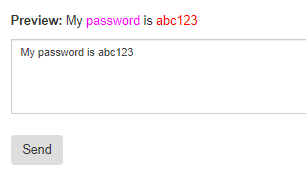
\includegraphics[width=1.0\textwidth]{Preview.png}

\begin{flushleft}
	Click send to submit your query. Queries will be handled and responded to by the system.
\end{flushleft}
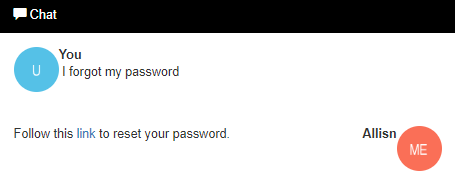
\includegraphics[width=1.0\textwidth]{Response.png}

\begin{flushleft}
	Follow the link to find the requested information.
	To login to a client representative account, click “Sign in” in the top right corner.
\end{flushleft}
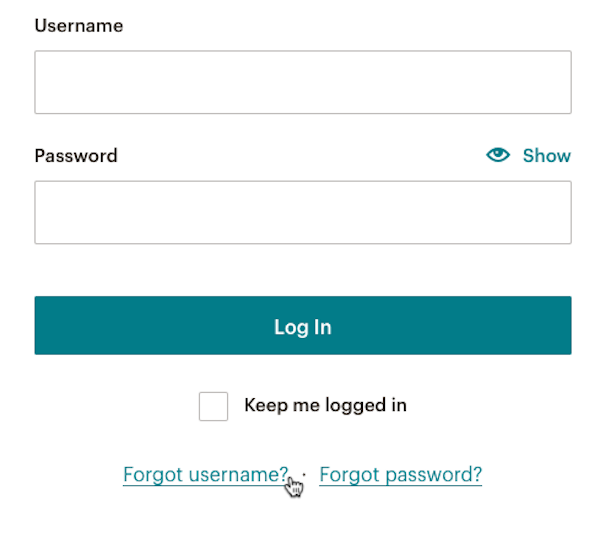
\includegraphics[width=1.0\textwidth]{Login.png}

\begin{flushleft}
	You will be redirected to the AuthO sign in page.
\end{flushleft}
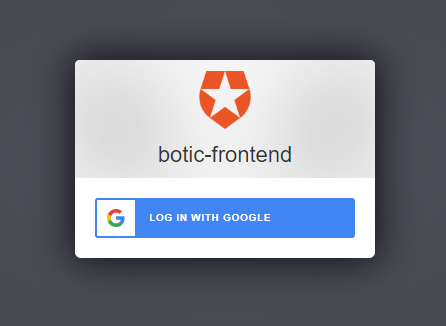
\includegraphics[width=1.0\textwidth]{AuthO.png}

\begin{flushleft}
	After signing into your account, you will be redirected to file:///C:/Users/Kyle/Documents/GitHub/Botic/ui/RepHome.html
\end{flushleft}
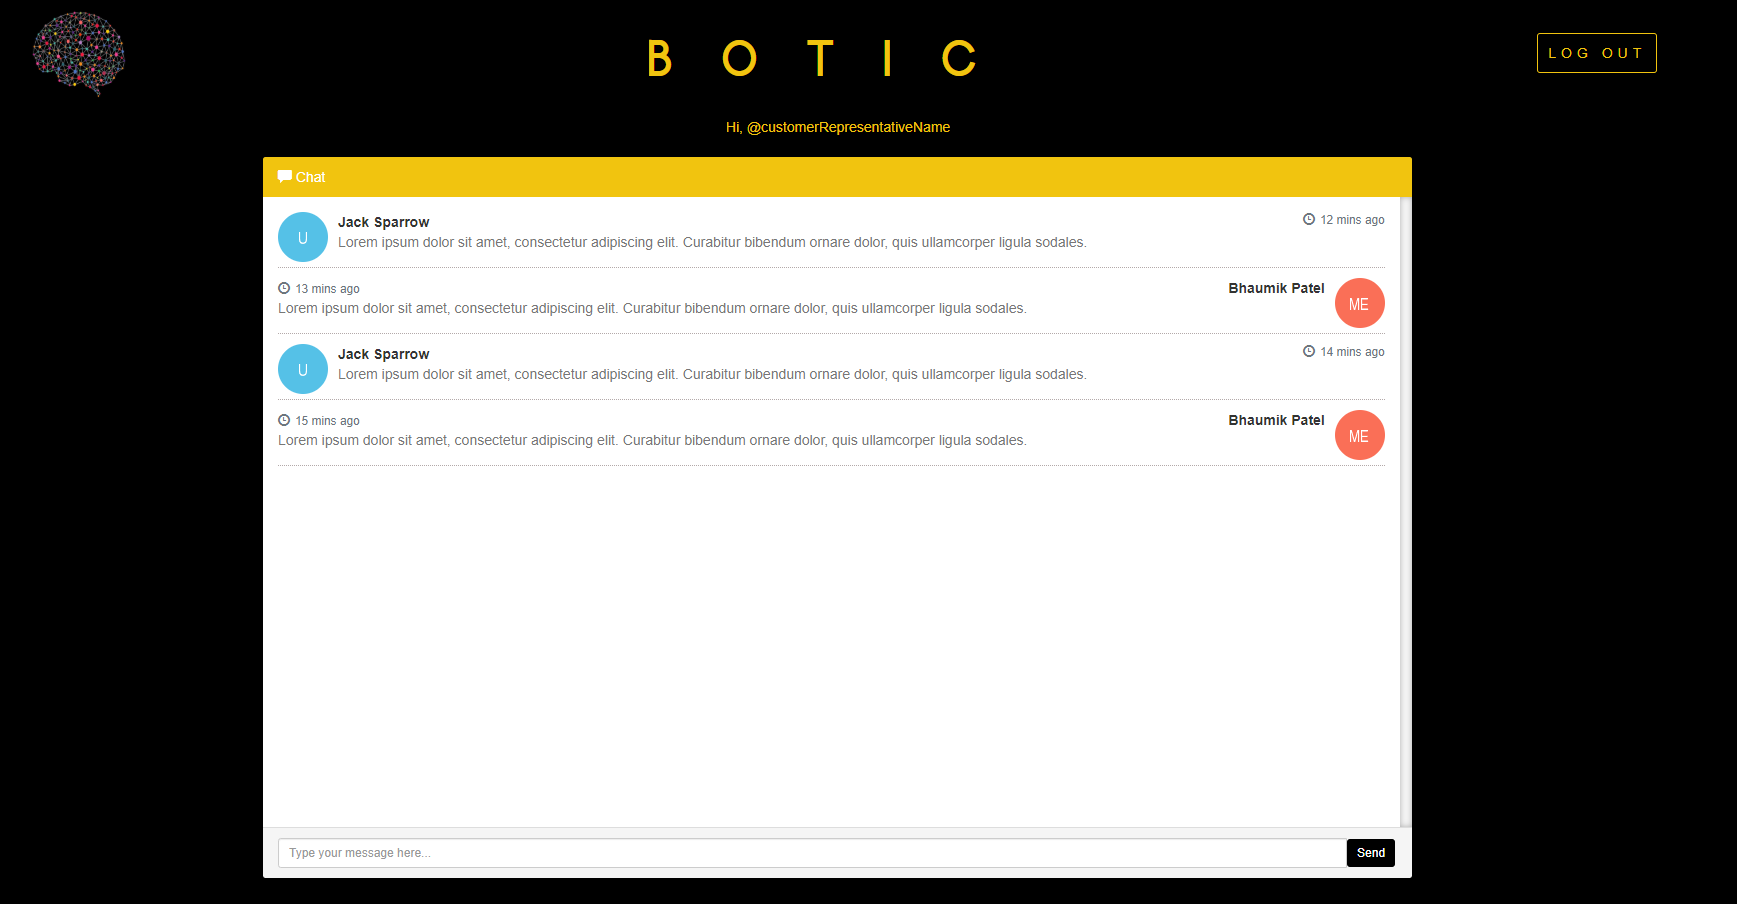
\includegraphics[width=1.0\textwidth]{Rep.png}

\begin{flushleft}
	Queries that could not be handled by the system will appear here for the client representative to review and respond to.
	Click “Log out” to logout of your account.
\end{flushleft}

\includegraphics[width=1.0\textwidth]{LogOut.png}

\begin{flushleft}
	Then confirm that you want to log out by clicking “Yes”.
\end{flushleft}
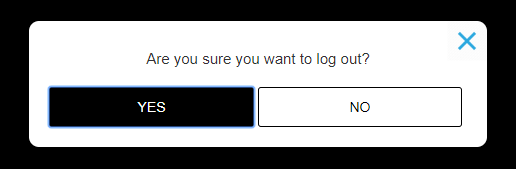
\includegraphics[width=1.0\textwidth]{Confirm.png}

\begin{flushleft}
You will be returned to file:///C:/Users/Kyle/Documents/GitHub/Botic/ui/landingPage.html
\end{flushleft}

\section{Troubleshooting}
What follows is a list of possible error conditions that may occur during the deployment and/or usage of your Botic instance as well as a number of ways we recommend they be dealt with.

\subsection{Deployment}
\begin{itemize}
    \item \textbf{Software doesn't install:} Check that you meet all of the prerequisites and that none of the packages installed were corrupted. During the download process
    \item \textbf{Software doesn't run:} Check the dockerfile and the angular build to ensure that all of the necessary prerequisite packages were installed.
    \item \textbf{API calls return errors during runtime:} Ensure that your deployment environment is configured to allow cross-origin http requests.
\end{itemize}

\subsection {Usage}
\begin{itemize}
        \item \textbf{Bot does not respond.} Check your connection and ensure that the communication port that BOTIC communicates on is exposed.
        \item\textbf{Bot is not highlighting information.} Check your connection to make sure information is being sent. Otherwise, ensure that your server is configured to allow BOTIC to make HTTP requests.
        \item \textbf{Bot is giving incoherent responses.}Check your training data as well as your information digest in to see if it is loaded correctly and that your model is properly trained.
\end{itemize}

\end{document}
